\section{Chi tiết thực hiện}
\subsection{Các thư viện cần thiết}
Trong đồ án này, các thư viện chính được sử dụng bao gồm:
\begin{itemize}
	\item \textbf{pandas}: Thư viện mạnh mẽ để thao tác và phân tích dữ liệu dạng bảng (DataFrame). Hỗ trợ đọc/ghi dữ liệu từ nhiều định dạng (CSV, Excel, SQL, v.v.), xử lý dữ liệu thiếu, và thực hiện các thao tác nhóm, lọc, sắp xếp.
	\item \textbf{numpy}: Thư viện xử lý mảng số học hiệu năng cao, cung cấp các phép tính toán vector hóa và đại số tuyến tính, hỗ trợ tối ưu tốc độ xử lý dữ liệu.
	\item \textbf{matplotlib}: Thư viện vẽ đồ thị 2D, được dùng để hiển thị biểu đồ, trực quan hóa kết quả phân tích dữ liệu.
	\item \textbf{seaborn}: Thư viện trực quan hóa dữ liệu dựa trên matplotlib, cung cấp các biểu đồ thống kê đẹp mắt và dễ tùy chỉnh, được dùng cho các biểu đồ như countplot, heatmap, pairplot.
	\item \textbf{IPython.display}: Cung cấp các hàm hỗ trợ hiển thị đối tượng trực tiếp trong môi trường Jupyter Notebook, đặc biệt hữu ích để hiển thị bảng dữ liệu đẹp mắt.
	\item \textbf{typing} (\texttt{Dict}, \texttt{Any}): Cung cấp các kiểu dữ liệu mạnh mẽ giúp mã dễ đọc và bảo trì.
\end{itemize}

\subsection{Yêu cầu 1: Phân tích khám phá dữ liệu (EDA)}
\subsubsection{Các hàm chính}

\begin{itemize}
	\item \textbf{ds\_overview(df)}: Trả về bảng tổng quan dữ liệu, bao gồm số dòng và số cột của DataFrame.
	\item \textbf{dtypes\_table(df)}: Trả về tên cột và kiểu dữ liệu của từng cột trong DataFrame.
	\item \textbf{uniques\_table(df)}: Thống kê số lượng giá trị duy nhất của mỗi cột, sắp xếp theo thứ tự giảm dần.
	\item \textbf{missing\_table(df)}: Thống kê số lượng và tỷ lệ phần trăm giá trị thiếu (NaN) trong mỗi cột.
	\item \textbf{duplicates\_table(df)}: Thống kê số lượng bản ghi trùng lặp trong DataFrame.
	\item \textbf{sample\_values(df, k)}: Lấy $k$ giá trị không null đầu tiên của mỗi cột, hiển thị dưới dạng bảng.
	\item \textbf{head\_tail(df, n)}: Trả về $n$ dòng đầu và $n$ dòng cuối của DataFrame.
	\item \textbf{remove\_duplicates(X\_df, y\_series)}: Loại bỏ các bản ghi trùng lặp trong DataFrame và Series, trả về DataFrame và Series đã loại bỏ trùng lặp.
	\item \textbf{eda\_overview(X, y)}: Thực hiện tổng hợp EDA ở mức metadata cho cả tập đặc trưng \texttt{X} và biến mục tiêu \texttt{y}.
	\item \textbf{plot\_histograms(df, bins, exclude)}: Vẽ histogram cho các cột số, loại trừ các cột chỉ định.
	\item \textbf{plot\_countplot(df, col)}: Vẽ countplot cho một cột phân loại.
	\item \textbf{plot\_scatter\_vs\_target(df, features, target)}: Vẽ scatter plot giữa từng đặc trưng số và biến mục tiêu.
	\item \textbf{plot\_correlation\_heatmap(df)}: Vẽ heatmap hiển thị ma trận tương quan giữa các biến số.
	\item \textbf{plot\_pairwise\_product\_correlation\_heatmap(df, target)}: Vẽ heatmap tương quan giữa tất cả các tích cặp đặc trưng và biến mục tiêu.
	\item \textbf{plot\_boxplots(df, features, target)}: Vẽ boxplot của từng đặc trưng so với biến mục tiêu, tự động binning nếu là dữ liệu số.
	\item \textbf{plot\_pairplot(df)}: Vẽ pairplot giữa tất cả các đặc trưng và biến mục tiêu.
	\item \textbf{plot\_all\_charts(df, target)}: Hàm tổng hợp, lần lượt gọi tất cả các hàm vẽ biểu đồ trên để thực hiện EDA toàn diện.
\end{itemize}

\subsubsection{Khám phá tổng quan dữ liệu}
\begin{table}[H]
	\centering
	\begin{tabular}{|c|l|c|}
		\hline
		\textbf{} & \textbf{Property} & \textbf{Value} \\ \hline
		0         & Number of rows    & 9000           \\
		1         & Number of columns & 6              \\ \hline
	\end{tabular}
	\caption{Tổng quan dữ liệu cho thấy dữ liệu có 9000 dòng và 6 cột.}
\end{table}

\begin{table}[H]
	\centering
	\begin{tabular}{|c|l|l|l|}
		\hline
		\textbf{} & \textbf{column}                  & \textbf{dtype} & \textbf{description}   \\ \hline
		0         & Hours Studied                    & int64          & Số giờ học tập         \\
		1         & Previous Scores                  & int64          & Điểm số trước đó       \\
		2         & Extracurricular Activities       & int64          & Hoạt động ngoại khóa   \\
		3         & Sleep Hours                      & int64          & Số giờ ngủ             \\
		4         & Sample Question Papers Practiced & int64          & Số lượng đề thi đã làm \\
		5         & Performance Index                & float64        & Chỉ số hiệu suất       \\ \hline
	\end{tabular}
	\caption{Kiểu dữ liệu các cột (các đặc trưng)}
\end{table}

\begin{table}[H]
	\centering
	\begin{tabular}{|c|l|c|}
		\hline
		\textbf{} & \textbf{column}                  & \textbf{nunique} \\ \hline
		0         & Performance Index                & 91               \\
		1         & Previous Scores                  & 60               \\
		2         & Sample Question Papers Practiced & 10               \\
		3         & Hours Studied                    & 9                \\
		4         & Sleep Hours                      & 6                \\
		5         & Extracurricular Activities       & 2                \\ \hline
	\end{tabular}
	\caption{Số lượng giá trị duy nhất của mỗi cột}
\end{table}

\begin{table}[H]
	\centering
	\begin{tabular}{|c|l|c|c|}
		\hline
		\textbf{} & \textbf{column}                  & \textbf{missing\_count} & \textbf{missing\_\%} \\ \hline
		0         & Hours Studied                    & 0                       & 0.0                  \\
		1         & Previous Scores                  & 0                       & 0.0                  \\
		2         & Extracurricular Activities       & 0                       & 0.0                  \\
		3         & Sleep Hours                      & 0                       & 0.0                  \\
		4         & Sample Question Papers Practiced & 0                       & 0.0                  \\
		5         & Performance Index                & 0                       & 0.0                  \\ \hline
	\end{tabular}
	\caption{Số lượng và tỷ lệ phần trăm giá trị thiếu}
\end{table}

\begin{table}[H]
	\centering
	\begin{tabular}{|c|c|}
		\hline
		\textbf{n\_duplicates} & \textbf{pct\_duplicates} \\ \hline
		103                    & 1.144                    \\ \hline
	\end{tabular}
	\caption{Số lượng và tỷ lệ phần trăm dòng trùng lặp}
\end{table}

Phân tích cho thấy có 103 dòng trùng lặp trong tập dữ liệu, chiếm 1,144\% tổng số dòng. Mặc dù tỷ lệ này không cao, nhưng để đảm bảo chất lượng phân tích và độ chính xác của mô hình, các bản ghi trùng lặp này đã được loại bỏ trước khi tiến hành các phân tích tiếp theo. Việc loại bỏ dữ liệu trùng lặp giúp tránh tình trạng các mẫu trùng lặp được đánh trọng số quá cao trong quá trình huấn luyện mô hình, từ đó nâng cao tính đại diện và độ tin cậy của mô hình hồi quy tuyến tính được xây dựng.

\subsubsection{Phân tích đơn biến}
Để thực hiện phân tích đơn biến, chúng ta sẽ xem xét từng đặc trưng một cách riêng biệt và lựa chọn các biểu đồ phù hợp để trực quan hóa phân phối của chúng. Các biểu đồ được sử dụng ở phần này bao gồm histogram, countplot:

\begin{figure}[H]
	\centering
	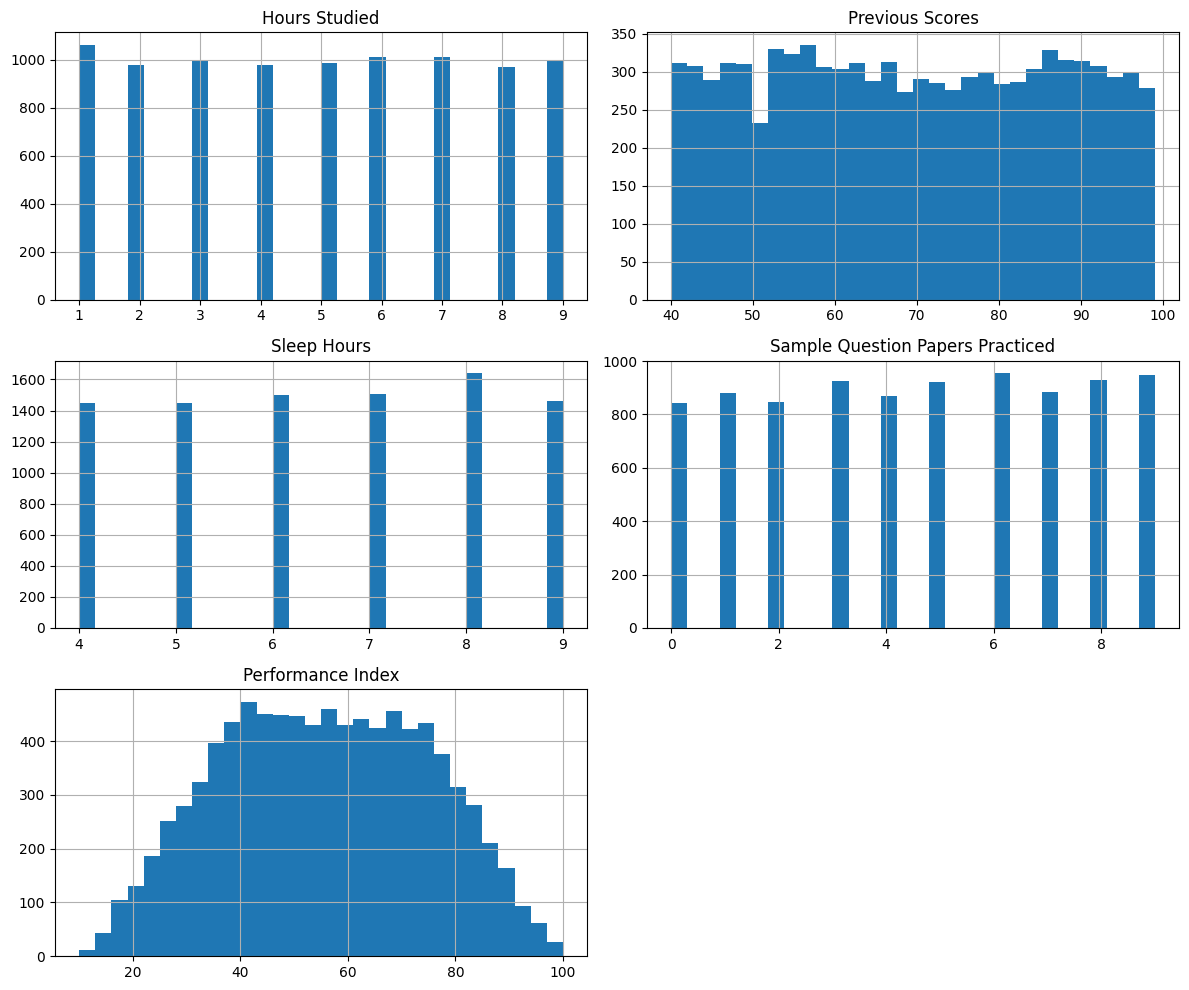
\includegraphics[width=\textwidth]{images/eda/1.png}
	\caption{Biểu đồ phân phối của các đặc trưng số}
\end{figure}

Phân phối của Hours Studied, Previous Scores, Sleep Hours và Sample Question Papers Practiced đều cho thấy sự phân bố khá đồng đều, ngoại trừ Performance Index có dạng phân phối chuẩn rõ rệt.

Điều này cho thấy thói quen học tập và thời gian ngủ của sinh viên nhìn chung ổn định, không tạo ra những giá trị ngoại lệ đáng kể về thành tích. Vì vậy, nhiều khả năng còn tồn tại các yếu tố khác ảnh hưởng đến sự biến động của Performance Index.

Dạng phân phối chuẩn của Performance Index cũng phản ánh rằng phần lớn sinh viên đạt mức thành tích trung bình, trong khi chỉ một số ít vượt trội hoặc tụt lại so với mặt bằng chung.

\begin{figure}[H]
	\centering
	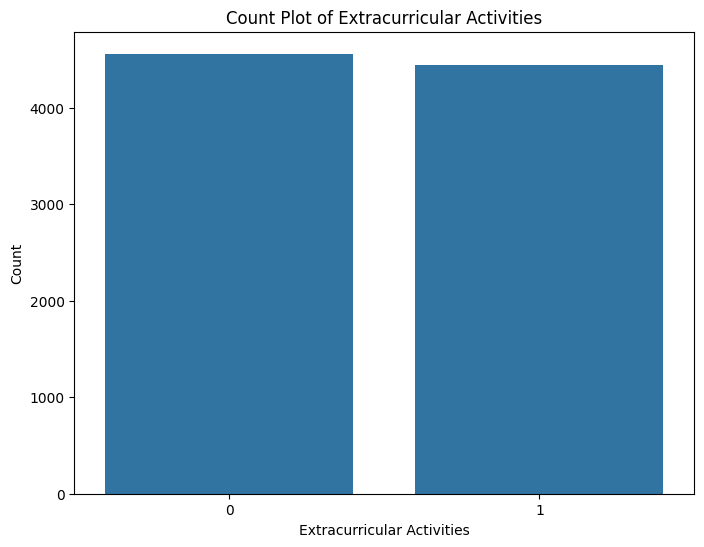
\includegraphics[width=0.8\textwidth]{images/eda/2.png}
	\caption{Biểu đồ countplot cho các đặc trưng phân loại}
\end{figure}

Kết quả phân tích cho thấy tỷ lệ sinh viên tham gia và không tham gia các hoạt động ngoại khóa gần như tương đương nhau.

Điều này phản ánh rằng các hoạt động ngoại khóa hiện nay đã đạt được mức độ tiếp cận tốt và thu hút được sự quan tâm của một bộ phận đáng kể sinh viên.

Tuy nhiên, vẫn tồn tại tiềm năng để mở rộng mức độ tham gia, thông qua việc đa dạng hóa loại hình hoạt động, nâng cao tính hấp dẫn hoặc đẩy mạnh công tác truyền thông nhằm khuyến khích nhiều sinh viên hơn tích cực tham gia.

\subsubsection{Phân tích hai biến}
Để hiểu rõ hơn về mối quan hệ giữa các đặc trưng và biến mục tiêu (Performance Index), chúng ta sẽ sử dụng scatter plot, heatmap và boxplot.

\begin{figure}[H]
	\centering
	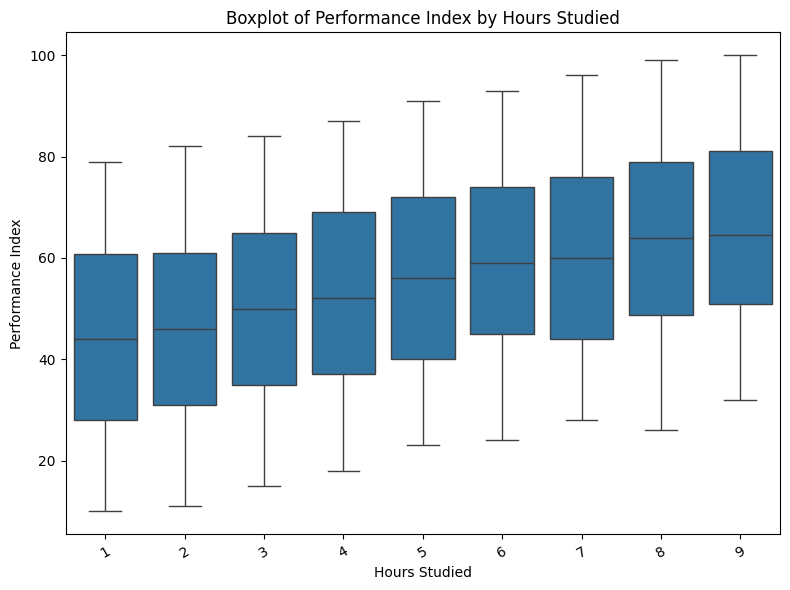
\includegraphics[width=0.8\textwidth]{images/eda/3.png}
	\caption{Biểu đồ boxplot giữa Performance Index và Hours Studied}
\end{figure}

Biểu đồ cho thấy trung vị điểm số tăng dần từ khoảng 45 (1 giờ học) lên 65 (9 giờ học), phản ánh mối quan hệ dương giữa thời gian học và thành tích.

Toàn bộ phân vị (Q1, Q3) dịch chuyển lên trên, nhưng độ phân tán lớn cho thấy kết quả vẫn chịu ảnh hưởng của nhiều yếu tố khác ngoài giờ học.

Ngoại lệ xuất hiện ở cả điểm rất thấp và rất cao ở mọi mức giờ học. Kết quả này phù hợp với hệ số tương quan dương vừa phải giữa Hours Studied và Performance Index, cho thấy nên giữ biến này và xem xét thêm các tương tác khi xây dựng mô hình.

\begin{figure}[H]
	\centering
	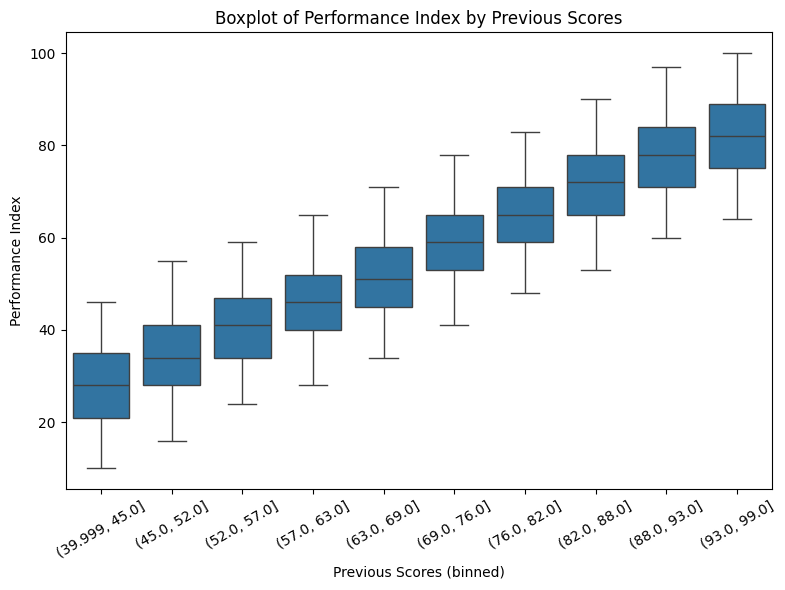
\includegraphics[width=0.8\textwidth]{images/eda/4.png}
	\caption{Biểu đồ boxplot giữa Performance Index và Previous Scores}
\end{figure}

Biểu đồ cho thấy trung vị của Performance Index tăng dần từ khoảng 25 (Previous Scores \~ 40) lên khoảng 85 (Previous Scores \~ 95), phản ánh mối quan hệ dương mạnh giữa điểm số trước đây và thành tích hiện tại.

Toàn bộ các phân vị (Q1, Q3) dịch chuyển lên trên khi Previous Scores tăng, đồng thời độ phân tán giảm ở nhóm điểm cao cho thấy sự ổn định hơn về kết quả ở các học sinh có nền tảng tốt.

Ngoại lệ vẫn xuất hiện ở cả mức rất thấp và rất cao trong mọi nhóm điểm, cho thấy rằng mặc dù Previous Scores là yếu tố quan trọng, vẫn tồn tại các yếu tố khác ảnh hưởng đến Performance Index. Kết quả này phù hợp với hệ số tương quan cao giữa Previous Scores và Performance Index, cho thấy biến này nên được giữ và có thể tạo thêm các biến tương tác hoặc biến phi tuyến khi xây dựng mô hình.

\begin{figure}[H]
	\centering
	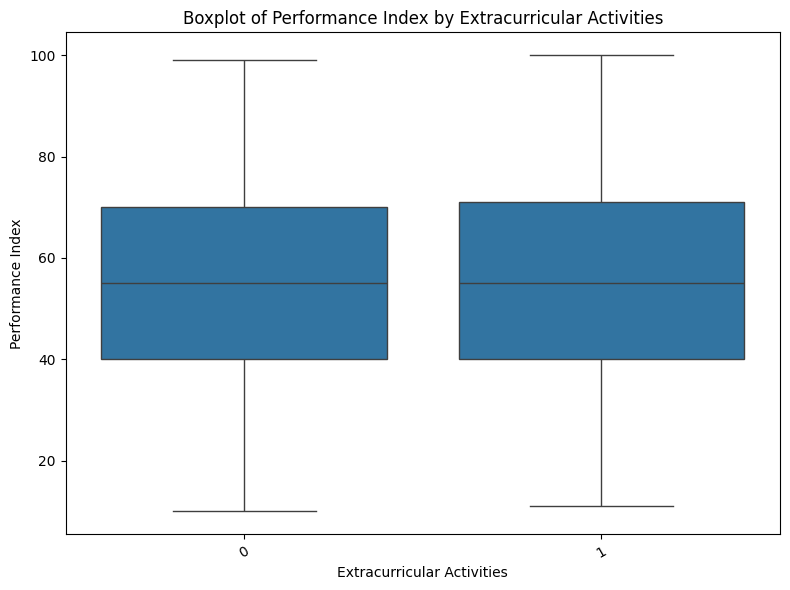
\includegraphics[width=0.8\textwidth]{images/eda/5.png}
	\caption{Biểu đồ boxplot giữa Performance Index và Extracurricular Activities}
\end{figure}

Biểu đồ cho thấy trung vị Performance Index của hai nhóm sinh viên tham gia và không tham gia hoạt động ngoại khóa gần như tương đương (\~55), phản ánh tác động hạn chế của yếu tố này đến thành tích học tập.

Phân vị của hai nhóm gần trùng nhau, cho thấy phân bố kết quả học tập tương đồng. Độ phân tán rộng cùng sự xuất hiện của các ngoại lệ ở cả hai nhóm cho thấy rằng thành tích chịu ảnh hưởng chủ yếu từ các yếu tố khác, không phải hoạt động ngoại khóa.

\begin{figure}[H]
	\centering
	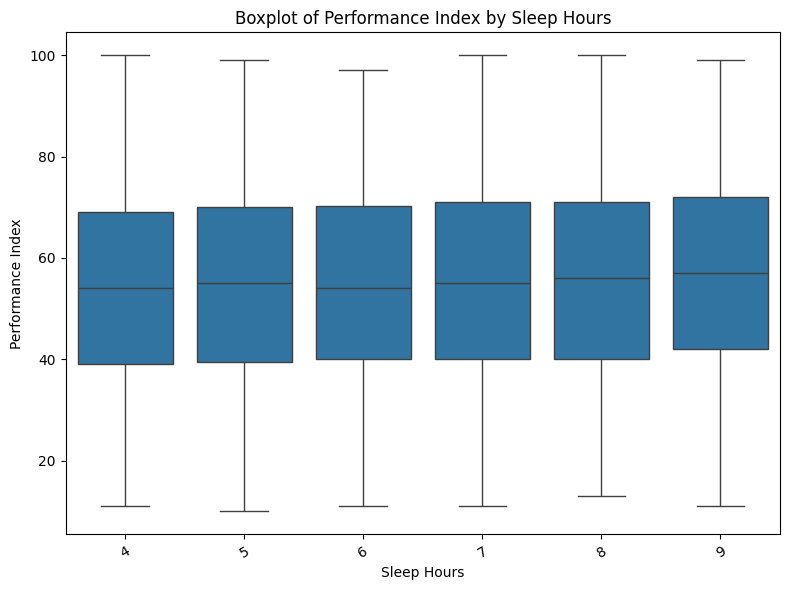
\includegraphics[width=0.8\textwidth]{images/eda/6.png}
	\caption{Biểu đồ boxplot giữa Performance Index và Sleep Hours}
\end{figure}

Biểu đồ cho thấy trung vị Performance Index dao động quanh mức 54 – 56 ở mọi mức giờ ngủ, cho thấy giấc ngủ không có mối quan hệ rõ rệt với thành tích học tập.

Các phân vị Q1 và Q3 gần như giữ nguyên, phản ánh phân bố kết quả tương đối ổn định giữa các nhóm. Độ phân tán rộng cùng sự xuất hiện của ngoại lệ ở cả hai đầu cho thấy các yếu tố khác ngoài giấc ngủ đóng vai trò quyết định hơn trong hiệu suất học tập.

\begin{figure}[H]
	\centering
	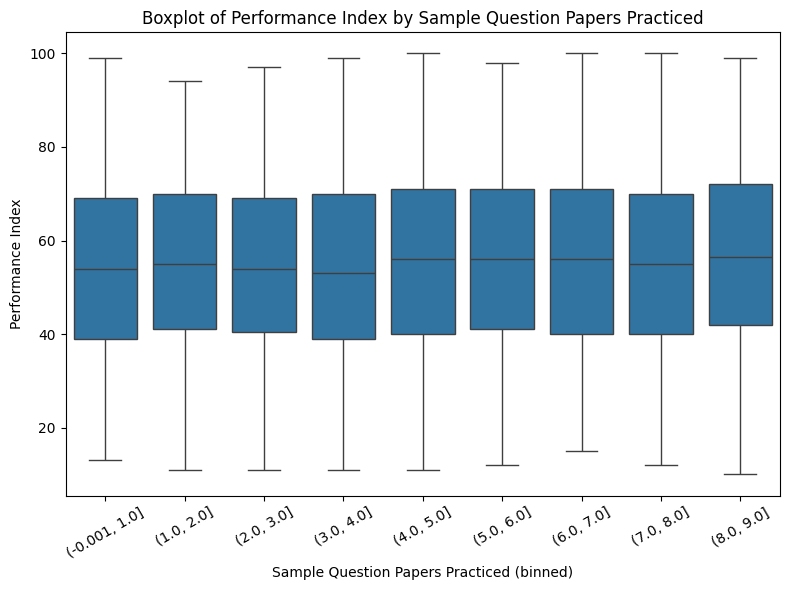
\includegraphics[width=0.8\textwidth]{images/eda/7.png}
	\caption{Biểu đồ boxplot giữa Performance Index và Sample Question Papers Practiced}
\end{figure}

Biểu đồ cho thấy trung vị Performance Index duy trì quanh mức 54 – 56 ở hầu hết các nhóm số lượng đề thi thử đã làm, cho thấy mối quan hệ yếu giữa biến này và thành tích học tập.

Khoảng phân vị Q1 – Q3 tương đối ổn định, trong khi độ phân tán rộng và sự xuất hiện của ngoại lệ ở cả hai đầu cho thấy yếu tố này chỉ đóng vai trò hỗ trợ, không phải là yếu tố quyết định chính đến Performance Index.

\begin{figure}[H]

	\centering
	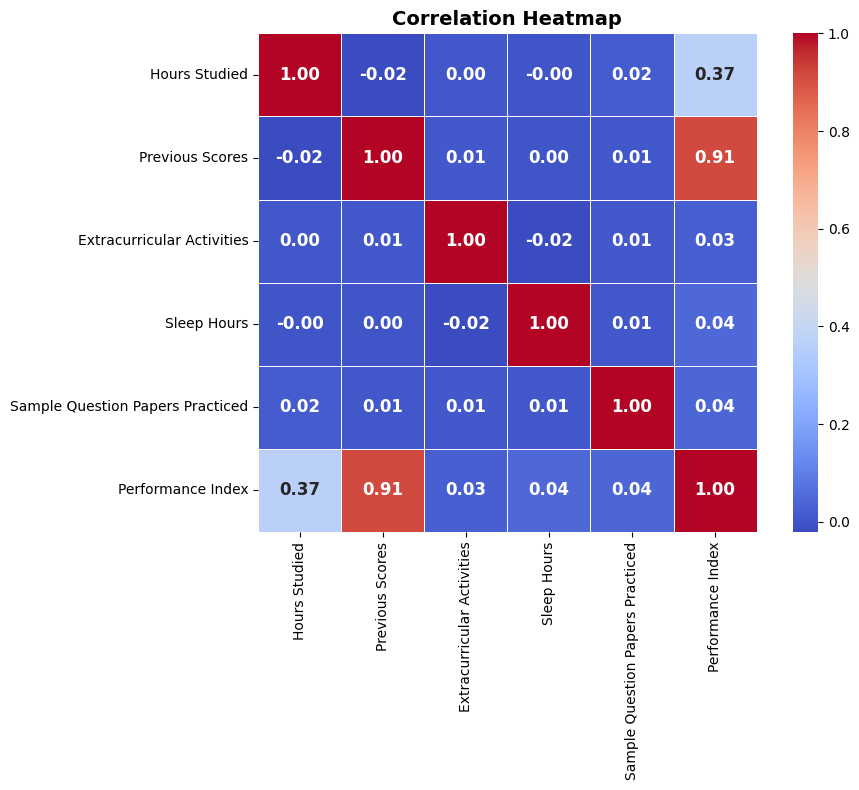
\includegraphics[width=\textwidth]{images/eda/8.png}
	\caption{Ma trận tương quan giữa các đặc trưng}
\end{figure}

Điểm số trước đây là yếu tố có ảnh hưởng lớn nhất đến Performance Index, nhấn mạnh tầm quan trọng của việc duy trì thành tích học tập tốt theo thời gian.

Số giờ học cũng có tác động tích cực đến Performance Index, nhưng mức độ ảnh hưởng không mạnh bằng thành tích học tập trước đó.

Các yếu tố khác như hoạt động ngoại khóa, giấc ngủ và luyện tập đề mẫu hầu như không tạo ra tác động đáng kể đến kết quả học tập. Trong đó, hoạt động ngoại khóa là biến có tương quan thấp nhất với Performance Index.

\begin{figure}[H]
	\centering
	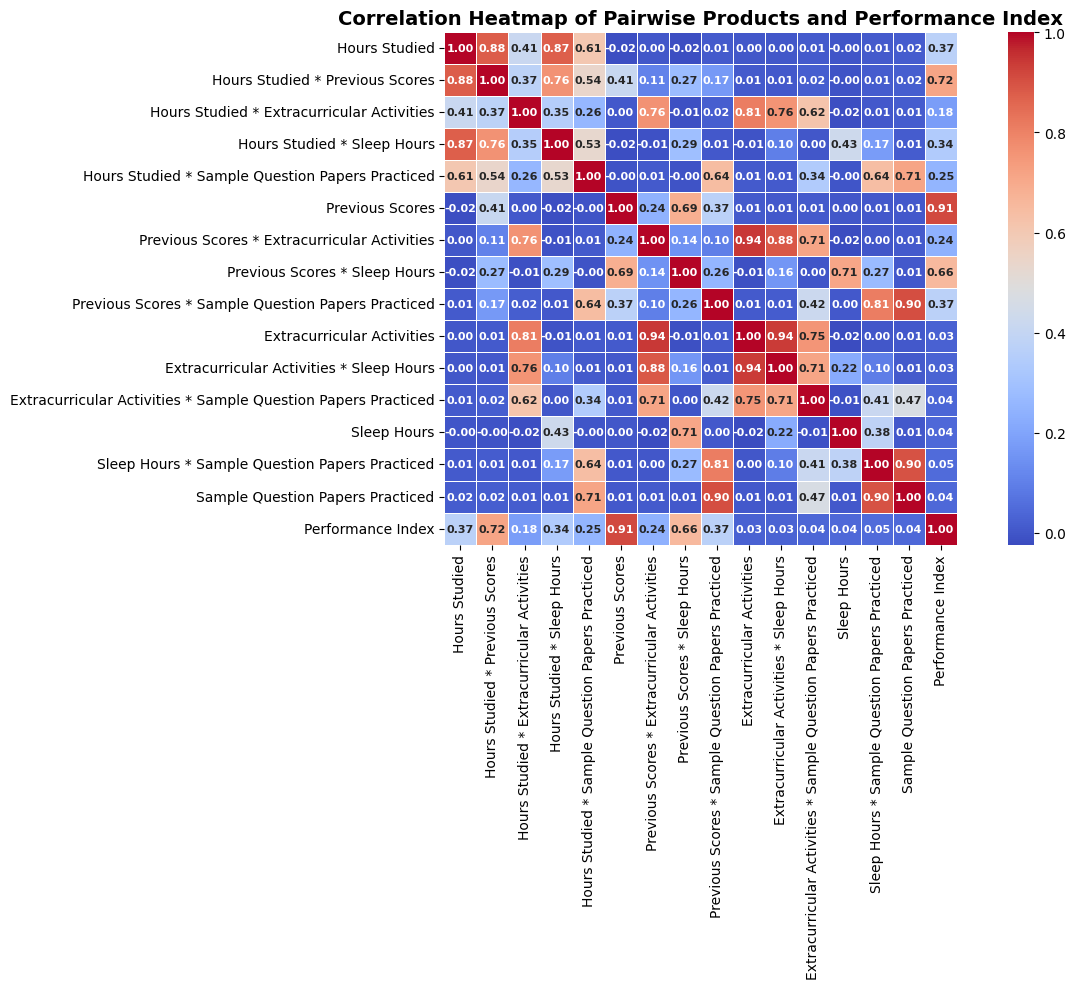
\includegraphics[width=\textwidth]{images/eda/9.png}
	\caption{Ma trận tương quan giữa các biến tương tác theo cặp}
\end{figure}

Ma trận tương quan mở rộng cho thấy ngoài các biến gốc, một số biến tương tác (pairwise products) có mức tương quan cao hơn với Performance Index so với khi xét riêng lẻ:
\begin{itemize}
	\item Previous Scores vẫn duy trì mức tương quan rất cao với Performance Index (0.91), tiếp tục khẳng định vai trò là yếu tố chính.
	\item Tương tác Previous Scores × Hours Studied đạt mức tương quan 0.72, cho thấy việc duy trì điểm số tốt kết hợp với học tập chăm chỉ có thể ảnh hưởng đến thành tích hiện tại.
	\item Hours Studied × Sleep Hours có tương quan 0.34, cao hơn so với xét riêng từng biến, cho thấy rằng sự cân bằng giữa thời gian học và ngủ có thể đóng góp tích cực.
\end{itemize}

\subsubsection{Phân tích nhiều biến}

\begin{figure}[H]
	\centering
	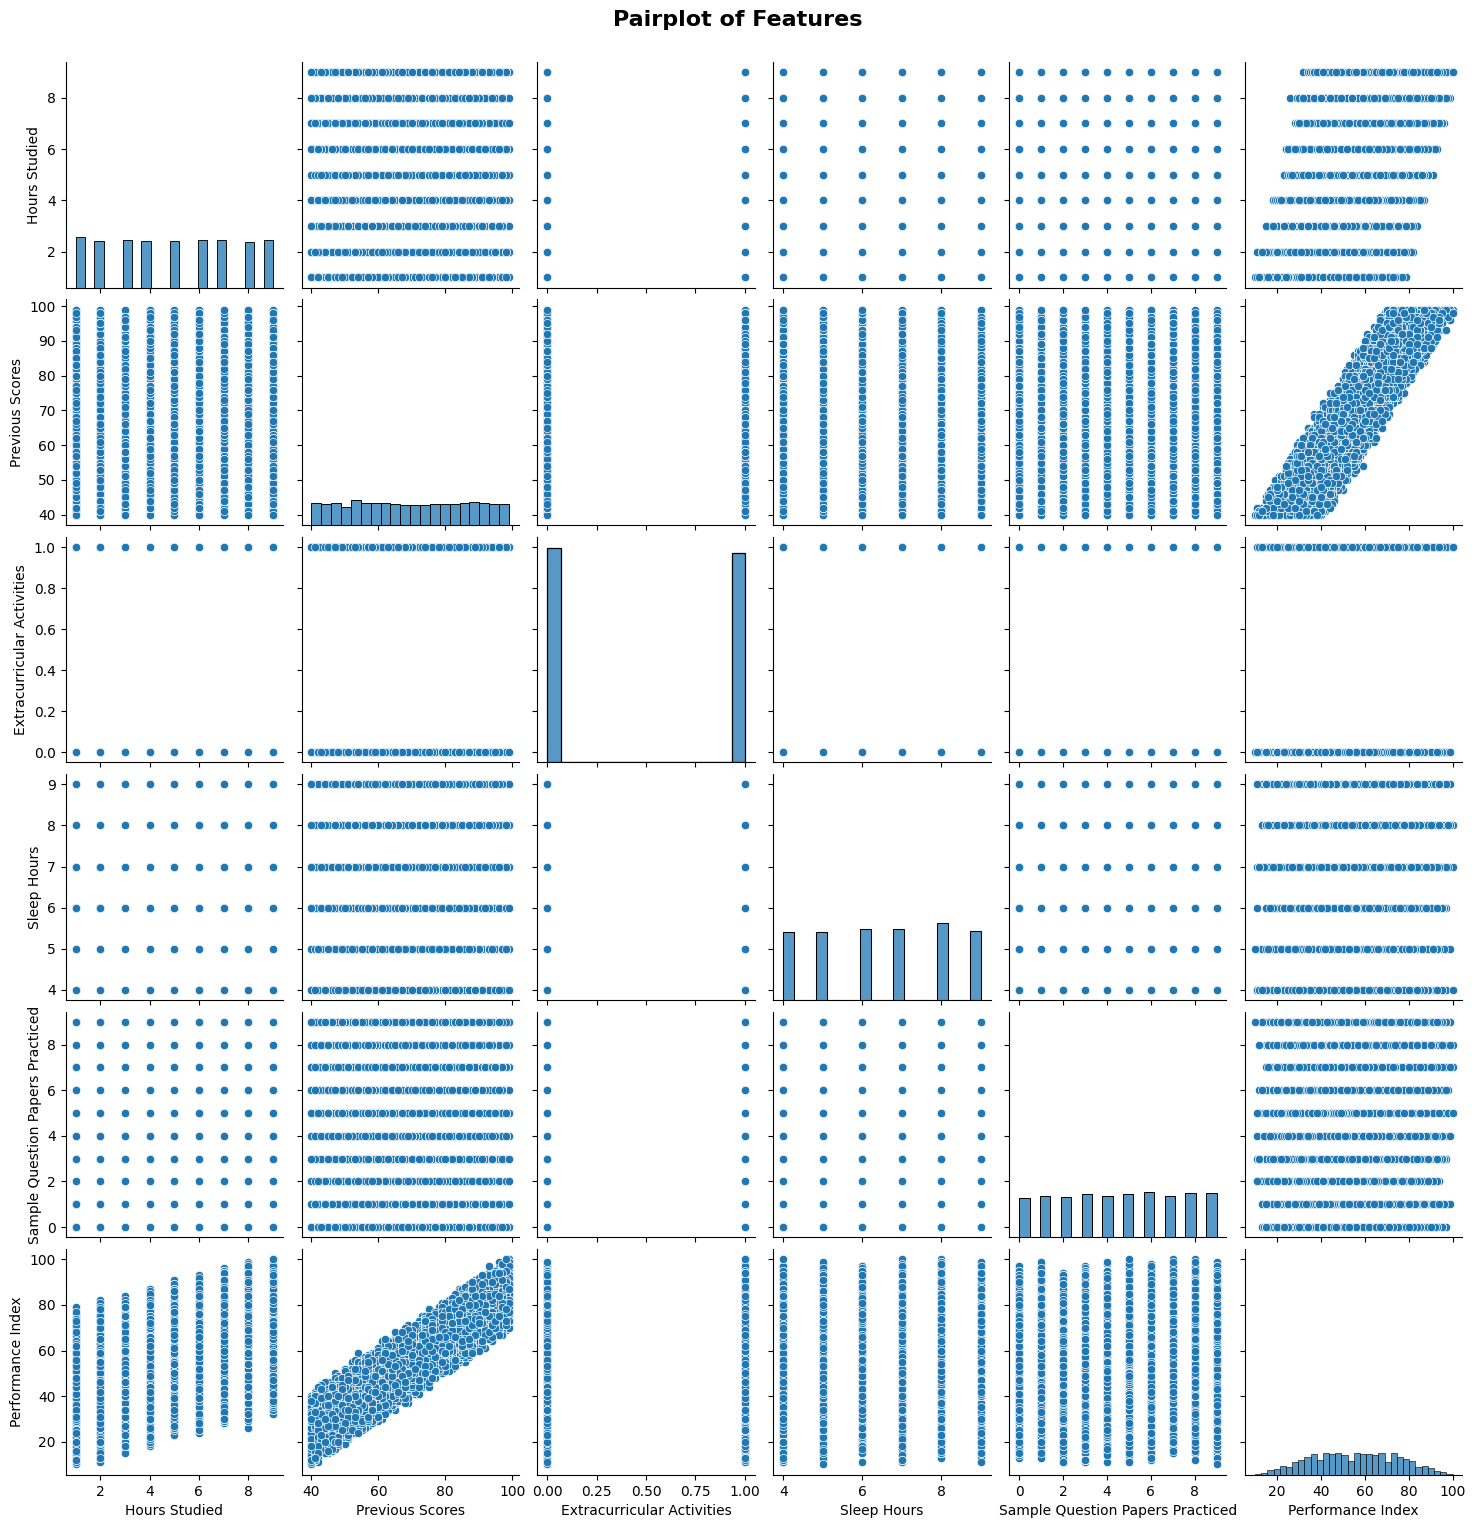
\includegraphics[width=\textwidth]{images/eda/10.png}
	\caption{Ma trận biểu đồ phân tán}
\end{figure}

\textbf{Mối quan hệ mạnh:} Mối quan hệ đáng kể và mạnh duy nhất được quan sát là giữa Previous Scores và Performance Index. Điều này nhất quán trên tất cả các biểu đồ và khẳng định rằng thành tích trong quá khứ là chỉ báo đáng tin cậy nhất cho thành tích trong tương lai trong bộ dữ liệu này.

\textbf{Mối quan hệ yếu:} Các yếu tố như Hours Studied, Extracurricular Activities, Sleep Hours và Sample Question Papers Practiced đều có mối quan hệ yếu với Performance Index. Điều này cho thấy rằng mặc dù chúng có thể ảnh hưởng đến thành tích, nhưng không phải là yếu tố quyết định chính.

\textbf{Phân phối của các đặc trưng: } Phân phối của các biến, đặc biệt là Performance Index và Previous Scores, cho thấy phạm vi giá trị rộng, phản ánh sự đa dạng trong thành tích học tập và điểm số trước đó của học sinh. Performance Index có xu hướng phân phối gần chuẩn, cho thấy phần lớn học sinh tập trung quanh mức trung bình, với số lượng ít hơn ở mức điểm rất cao hoặc rất thấp.

Nhìn chung, phân tích EDA cho thấy Previous Scores là yếu tố quan trọng nhất ảnh hưởng đến Performance Index, trong khi các yếu tố khác như Hours Studied và Sleep Hours có tác động phụ trợ. Các hoạt động ngoại khóa và luyện tập đề mẫu không có mối liên hệ rõ ràng với thành tích học tập.

\subsection{Yêu cầu 2a: Sử dụng toàn bộ 5 đặc trưng để xây dựng mô hình hồi quy tuyến tính}
\subsubsection{Các hàm hỗ trợ}

\begin{itemize}
	\item \textbf{train\_linear\_regression(X, y):} Hàm này huấn luyện mô hình hồi quy tuyến tính sử dụng công thức giải tích (Normal Equation). Đầu vào là ma trận đặc trưng \( X \) và vector mục tiêu \( y \). Các bước thực hiện bao gồm:
	      \begin{enumerate}
		      \item Tạo ma trận mở rộng bằng cách thêm một cột các giá trị 1 để xử lý hệ số tự do:
		            \begin{equation}
			            X_{\text{aug}} = [X | \mathbf{1}]
		            \end{equation}

		      \item Áp dụng công thức Normal Equation để tìm các hệ số tối ưu:
		            \begin{equation}
			            w_{\text{full}} = (X_{\text{aug}}^T X_{\text{aug}})^{-1} X_{\text{aug}}^T y
		            \end{equation}

		      \item Tách vector kết quả thành trọng số \( w \) cho các đặc trưng và hệ số tự do \( b \):
		            \begin{equation}
			            w = w_{\text{full}}[:-1], \quad b = w_{\text{full}}[-1]
		            \end{equation}
	      \end{enumerate}

	\item \textbf{mean\_squared\_error(y\_true, y\_pred):} Hàm tính sai số bình phương trung bình (MSE) giữa giá trị thực tế và dự đoán. Cài đặt bằng numpy thông qua lệnh \texttt{np.mean((y\_true - y\_pred)**2)}. MSE luôn không âm và càng nhỏ thì mô hình càng chính xác.

\end{itemize}

\subsubsection{Huấn luyện mô hình}
Sau khi cài đặt các hàm cần thiết, tiến hành huấn luyện mô hình hồi quy tuyến tính sử dụng toàn bộ 5 đặc trưng:

\begin{enumerate}
	\item Chuyển đổi dữ liệu X\_train và y\_train thành mảng numpy để thực hiện các phép toán hiệu quả
	\item Huấn luyện mô hình bằng hàm \texttt{train\_linear\_regression} để tìm vector trọng số \(w\) và hệ số tự do \(b\)
	\item Xây dựng công thức hồi quy tuyến tính dựa trên các trọng số tìm được
	\item Thực hiện dự đoán trên tập kiểm tra và đánh giá hiệu suất bằng MSE
\end{enumerate}

\subsection{Yêu cầu 2b: Xây dựng mô hình sử dụng duy nhất 1 đặc trưng, tìm mô hình cho kết quả tốt nhất}
\subsubsection{Các hàm hỗ trợ}
\begin{itemize}
	\item \textbf{manual\_shuffle(X\_df, y\_series):} Hàm này trộn ngẫu nhiên các hàng của DataFrame đặc trưng và Series mục tiêu theo cùng một thứ tự để đảm bảo tính tương thích:
	      \begin{enumerate}
		      \item Tạo mảng chỉ số từ 0 đến số lượng mẫu: \texttt{idx = np.arange(len(X\_df))}
		      \item Xáo trộn ngẫu nhiên chỉ số bằng numpy: \texttt{np.random.shuffle(idx)}
		      \item Áp dụng chỉ số đã xáo trộn để tái sắp xếp dữ liệu và đặt lại chỉ mục
	      \end{enumerate}

	\item \textbf{cross\_validate\_features(X, y, feature\_names, k=5):} Thực hiện k-fold cross-validation cho từng đặc trưng riêng biệt:
	      \begin{enumerate}
		      \item Chia dữ liệu thành \(k\) phần bằng nhau
		      \item Với mỗi đặc trưng, lần lượt sử dụng \(k-1\) phần làm tập huấn luyện và 1 phần làm tập kiểm định
		      \item Huấn luyện mô hình hồi quy tuyến tính một chiều và tính MSE trên tập kiểm định
		      \item Tính trung bình MSE qua \(k\) lần lặp cho mỗi đặc trưng
	      \end{enumerate}

	\item \textbf{display\_cv\_table(results):} Hiển thị kết quả cross-validation dưới dạng bảng tóm tắt với các cột: STT, tên đặc trưng và MSE trung bình.

	\item \textbf{display\_fold\_detail\_table(results, k=5):} Hiển thị bảng chi tiết MSE cho từng fold và từng đặc trưng, với hàng là tên đặc trưng, cột là số fold và MSE trung bình.
\end{itemize}

\subsubsection{Đánh giá và lựa chọn đặc trưng tối ưu}
Để tìm đặc trưng đơn lẻ tốt nhất, chúng tôi tiến hành quá trình đánh giá và lựa chọn thông qua 3 bước chính:

\begin{enumerate}
	\item \textbf{Đánh giá đặc trưng bằng k-fold cross-validation:}
	      \begin{itemize}
		      \item Trộn ngẫu nhiên dữ liệu huấn luyện bằng hàm \texttt{manual\_shuffle}
		      \item Thực hiện cross-validation với $k=5$ cho từng đặc trưng
		      \item Hiển thị bảng tổng hợp MSE và chi tiết từng fold để so sánh hiệu năng
		      \item Xác định đặc trưng có MSE trung bình thấp nhất (\texttt{Previous Scores})
	      \end{itemize}

	\item \textbf{Huấn luyện mô hình tốt nhất:}
	      \begin{itemize}
		      \item Chọn đặc trưng tốt nhất từ tập huấn luyện bằng MSE
		      \item Huấn luyện mô hình hồi quy tuyến tính (mô hình của đặc trưng tốt nhất) trên toàn bộ tập huấn luyện
		      \item Xây dựng công thức hồi quy tuyến tính dạng $y = wx + b$ với đặc trưng đã chọn
	      \end{itemize}

	\item \textbf{Đánh giá trên tập kiểm tra:}
	      \begin{itemize}
		      \item Áp dụng mô hình đã huấn luyện để dự đoán kết quả trên tập kiểm tra
		      \item Tính MSE để đánh giá hiệu năng cuối cùng
	      \end{itemize}
\end{enumerate}

\subsection{Yêu cầu 2c: Sinh viên tự xây dựng/thiết kế mô hình, tìm mô hình cho kết quả tốt nhất}
\subsubsection{Quy ước ký hiệu}
Các biến sau đây sẽ được sử dụng để thể hiện các đặc trưng trong bộ dữ liệu:
\begin{table}[H]
	\centering
	\begin{tabular}{|c|l|}
		\hline
		\textbf{Ký hiệu} & \textbf{Mô tả đặc trưng}                                  \\
		\hline
		$F_1$            & Hours Studied (Số giờ học tập)                            \\
		$F_2$            & Previous Scores (Điểm số trước đó)                        \\
		$F_3$            & Extracurricular Activities (Hoạt động ngoại khóa)         \\
		$F_4$            & Sleep Hours (Số giờ ngủ)                                  \\
		$F_5$            & Sample Question Papers Practiced (Số lượng đề thi đã làm) \\
		\hline
	\end{tabular}
	\caption{Quy ước ký hiệu cho các đặc trưng trong mô hình}
\end{table}

\subsubsection{Thiết kế và lựa chọn mô hình}

Dựa trên kết quả phân tích khám phá dữ liệu (EDA) từ yêu cầu 1, tôi đã thiết kế ba mô hình hồi quy tuyến tính với các lý do sau:

\textbf{Mô hình 1: Sử dụng 2 đặc trưng quan trọng nhất ($F_1$ và $F_2$)}
$$ \text{Student Performance} = \alpha_{0} + \alpha_{1}F_{1} + \alpha_{2}F_{2} $$

\begin{itemize}
	\item Từ ma trận tương quan (Hình 8), \textbf{Previous Scores} ($F_2$) có hệ số tương quan cao nhất với Performance Index (0.91), trong khi \textbf{Hours Studied} ($F_1$) có hệ số tương quan đứng thứ hai (0.37).
	\item Biểu đồ boxplot (Hình 3 và 4) cho thấy trung vị của Performance Index tăng rõ rệt theo cả hai đặc trưng này, đặc biệt là Previous Scores với mức tăng từ khoảng 25 (Previous Scores \~40) lên khoảng 85 (Previous Scores \~95).
	\item Mô hình này áp dụng nguyên tắc tiết kiệm (parsimony) bằng cách sử dụng số lượng tối thiểu các đặc trưng có tác động mạnh nhất, tránh overfitting.\cite{parsimony}
\end{itemize}

\textbf{Mô hình 2: Loại bỏ $F_3$, thêm bình phương của $F_2$}
$$ \text{Student Performance} = \alpha_{0} + \alpha_{1}F_{1} + \alpha_{2}F_{2} + \alpha_{3}F_{4} + \alpha_{4}F_{5} + \alpha_{5}F_{2}^2 $$

\begin{itemize}
	\item Ma trận tương quan (Hình 8) cho thấy \textbf{Extracurricular Activities} ($F_3$) có hệ số tương quan thấp nhất (0.03) với Performance Index.
	\item Biểu đồ boxplot (Hình 5) xác nhận rằng trung vị Performance Index gần như giống nhau (\~55) giữa nhóm tham gia và không tham gia hoạt động ngoại khóa nên loại bỏ.
	\item Biểu đồ phân tán (Hình 10) có thể thấy mối quan hệ tuyến tính giữa Previous Scores và Performance Index. Ngoài ra, thêm biến bình phương của $F_2$ ($F_2^2$) vào mô hình giúp kiểm tra mối quan hệ phi tuyến trong mô hình. Việc này giúp mô hình nắm bắt tốt hơn mối quan hệ phi tuyến nếu có tồn tại.
	\item Sleep Hours ($F_4$) và Sample Question Papers Practiced ($F_5$) được giữ lại vì chúng có thể đóng góp nhỏ nhưng có ý nghĩa khi kết hợp với các đặc trưng khác.
\end{itemize}

\textbf{Mô hình 3: Sử dụng đặc trưng tương tác ($F_1 \times F_2$)}
$$ \text{Student Performance} = \alpha_{0} + \alpha_{1}(F_{1} \times F_{2}) $$

\begin{itemize}
	\item Ma trận tương quan mở rộng (Hình 9) cho thấy tương tác \textbf{Hours Studied × Previous Scores} có hệ số tương quan cao (0.72) với Performance Index, cao hơn đáng kể so với Hours Studied đơn thuần (0.37).
	\item Điều này cho thấy rằng tác động của thời gian học có thể phụ thuộc vào điểm số trước đó: học sinh có nền tảng tốt có thể tận dụng hiệu quả hơn thời gian học.
	\item Mô hình tương tác này đơn giản với chỉ một biến dự đoán, nhưng vẫn có khả năng nắm bắt hiệu ứng kết hợp của hai đặc trưng quan trọng nhất.
\end{itemize}

Ba mô hình này thể hiện các phương pháp tiếp cận khác nhau dựa trên các hiểu biết từ EDA: từ mô hình đơn giản với các đặc trưng quan trọng nhất (Mô hình 1), mô hình mở rộng với biến phi tuyến (Mô hình 2), đến mô hình tập trung vào hiệu ứng tương tác (Mô hình 3). Việc so sánh hiệu suất của ba mô hình này sẽ giúp xác định phương pháp tiếp cận hiệu quả nhất cho bài toán dự đoán Performance Index.

\subsubsection{Các hàm hỗ trợ}

\begin{itemize}
	\item \textbf{create\_model1, create\_model2, create\_model3:} Ba hàm này tạo ra các DataFrame đặc trưng phù hợp với mỗi mô hình đề xuất:
	      \begin{itemize}
		      \item \texttt{create\_model1}: Chọn hai đặc trưng quan trọng nhất là Hours Studied và Previous Scores.
		      \item \texttt{create\_model2}: Thêm đặc trưng bình phương của Previous Scores và loại bỏ Extracurricular Activities.
		      \item \texttt{create\_model3}: Tạo đặc trưng tương tác giữa Hours Studied và Previous Scores.
	      \end{itemize}

	\item \textbf{define\_models:} Định nghĩa danh sách các mô hình cần đánh giá với tên, hàm tạo đặc trưng và mô tả.

	\item \textbf{cross\_validate\_custom\_model:} Thực hiện k-fold cross-validation cho một mô hình tùy chỉnh:
	      \begin{itemize}
		      \item Chia dữ liệu thành $k$ fold (mặc định $k=5$)
		      \item Với mỗi fold, tạo tập validation và tập training
		      \item Áp dụng hàm tạo đặc trưng cho cả hai tập dữ liệu
		      \item Huấn luyện mô hình và tính MSE trên tập validation
		      \item Tính trung bình MSE qua tất cả các fold
	      \end{itemize}

	\item \textbf{evaluate\_models:} Đánh giá tất cả mô hình trên cùng một dữ liệu đã xáo trộn:
	      \begin{itemize}
		      \item Trộn dữ liệu một lần duy nhất bằng \texttt{manual\_shuffle}
		      \item Đánh giá từng mô hình bằng \texttt{cross\_validate\_custom\_model}
		      \item Xác định mô hình tốt nhất dựa trên MSE trung bình thấp nhất
	      \end{itemize}

	\item \textbf{display\_model\_results:} Hiển thị kết quả đánh giá các mô hình:
	      \begin{itemize}
		      \item In thông báo về mô hình tốt nhất và MSE trung bình
		      \item Tạo bảng tổng kết với STT, tên mô hình và MSE
		      \item Hiển thị bảng chi tiết MSE từng fold cho từng mô hình
	      \end{itemize}

	\item \textbf{train\_best\_model:} Huấn luyện mô hình tốt nhất trên toàn bộ tập huấn luyện:
	      \begin{itemize}
		      \item Lấy tên và hàm tạo đặc trưng của mô hình tốt nhất
		      \item Áp dụng biến đổi đặc trưng cho tập huấn luyện và kiểm tra
		      \item Huấn luyện mô hình và trả về thông tin chi tiết
	      \end{itemize}

	\item \textbf{print\_regression\_formula:} In công thức hồi quy với các trọng số đã làm tròn.

	\item \textbf{evaluate\_on\_test\_set:} Đánh giá mô hình trên tập kiểm tra và in MSE.
\end{itemize}
